%!TEX root = Tesi__Simone_Mariotti.tex
\chapter{Visione Artificiale}
\fancyhead[R]{\bfseries Visione Artificiale} 	 	
\fancyfoot[C]{\thepage } 
La \textit{visione artificiale} ha come compito la creazione di 
un modello del mondo reale in tre dimensioni a partire da numerose 
immagini bidimensionali per cercare di emulare il processo biologico della vista.
Negli esseri umani, così come in molte altre specie, vedere non è solo scattare una 
fotografia bidimensionale mentale di un ambiente, ma è interpretare le informazioni
ricevute attraverso la retina per analizzare e creare un modello 3D dell'ambiente
circostante.\\	
Un sistema di visione artificiale, per provare ad avvicinarsi alla capacità visiva
e di interpretazione umana, ha bisogno di numerosi componenti di diversa natura: 
ottici, elettronici e meccanici per acquisire e memorizzare le immagini da elaborare.
Il primo tentativo in tal senso è datato 1883 quando  Paul Gottlieb Nipkow 
inventò il primo sistema in grado di trasformare informazioni visive in un segnale elettrico.\cite{Nipkow1} 
\\Il sistema si basa su un disco con dei fori praticati lungo una spirale che parte dal centro del disco
e procede verso l'esterno. Il disco ruota ad una velocità costante mentre l'immagine 
inquadrata viene focalizzata da una lente verso i fori in modo che un sensore, 
posto sul retro del disco, possa percepire i cambi di luminosità della porzione di scena
inquadrata e convertire questa variazione in segnali elettrici. 
\\Il ricevitore emetterà luce in base a dei 
segnali elettrici e attraverso un disco identico al primo e in rotazione sincrona 
proietterà un'immagine con tante righe quante sono i fori del disco.\cite{Nipkow2} 
Questo sistema porterà alla creazione della TV meccanica nel 1925.
\begin{figure}[!htb] \center
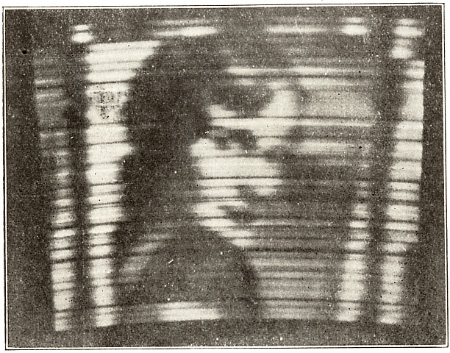
\includegraphics[width=\textwidth]{immagini/tv_meccanica.png}
\caption{Immagine visibile su una TV meccanica del 1925} 
\end{figure}
Negli anni successivi, con l'introduzione della miniaturizzazione nell'elettronica, 
sono stati compiuti enormi progressi. Da un punto di vista teorico, gli scienziati 
cominciarono ad ispirarsi al corpo umano nel tentativo di riprodurre il suo comportamento. Analizzando da vicino
l'occhio e in particolare la retina hanno scoperto che era formata da minuscoli 
recettori sensibili alla luce collegati al cervello tramite il nervo ottico. 
Si è così deciso di creare dei 
micro sensori di luce e formarne un'enorme matrice. Il primo risultato di questi studi 
si ebbe circa 40 anni dopo e fu il sensore CCD\footnote{Charge-Coupled Device.}, 
ideato da Willard S. Boyle e George E. Smith nel 1969 presso i Bell Laboratories,
mentre dobbiamo aspettare il 1993 per vedere i primi prototipi funzionanti del 
sensore CMOS\footnote{Complementary Metal-Oxide-Semiconductor.} sviluppati presso 
il Jet Propulsion Laboratory, entrambi hanno come elemento base il fotodiodo che 
equivale ad un pixel. Il CCD è un sensore 
analogico\footnote{Il sensore più grande esistente è di 1,4 Gigapixel ed è 
montato sul telescopio Pan-STARRS sviluppato per l'individuazione di meteoriti in
 rotta di collisione con la Terra.} che ha bisogno di più energia 
ma offre in genere una qualità superiore un rumore minore ad un costo più elevato.\\
\begin{figure}[!htb] \center
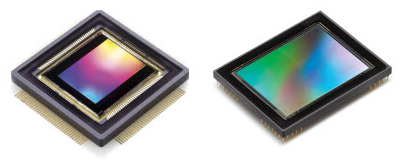
\includegraphics[scale=0.8]{immagini/ccd-cmos.png}
\caption{Due sensori moderni. A sinistra un sensore CMOS a destra uno CCD} 
\end{figure}
Il CMOS è un sensore digitale che offre una buona qualità di immagine ad costo minore;
per contro l'immagine presenta un forte rumore a causa della conversione 
analogico-digitale.\\
La visione artificiale ha principalmente tre utilizzi:
\begin{itemize}
\item \textbf{Ricognizione:} ricercare uno o più oggetti, scelti a priori, e organizzarli in 
insiemi generici o classi mantenendo informazioni riguardo il loro posizionamento 
nella scena. \\Esempio: ricercare in un'immagine o in un video tutte le persone, 
le macchine o gli animali. 
\item \textbf{Identificazione:} identificare una istanza specifica di una classe 
di oggetti. \\Esempio: ricercare in un'immagine o in un video un volto, 
una macchina o un animale specifico.. 
\item \textbf{Individuazione:} cercare una condizione specifica nell'immagine. 
\\Esempio: cercare imperfezioni nelle immagini a raggi X di superfici o materiali.
\end{itemize}
Un campo che ne fa massiccio utilizzo è la modellazione di ambienti 3D a partire 
da due o più immagini 2D; questo è stato reso possibile 
grazie all'enorme aumento della capacità di elaborazione grafica delle GPU.\\
La visione artificiale è stata applicata a molti altri campi nei quali si è verificata 
una vera e propria rivoluzione.

Uno di questi è la medicina nella quale l'introduzione di questa tecnica ha portato
all'analisi di radiografie, angiografie,
tomografie e altre immagini mediche. In questo modo è possibile identificare anomalie e 
problemi, quali i tumori, che non sarebbero visibili all'occhio umano 
se non in seguito a procedure molto invasive.

Un altro campo è quello del controllo di veicoli autonomi i quali stanno aumentando
ad un ritmo vertiginoso, progressivamente al migliorarsi delle tecniche di 
visione artificiale. Autovetture, droni, robot e carri per il rifornimento 
sono solo degli esempi a cosa può portare la visione artificiale applicata nei settori 
civili e di ricerca.
\begin{figure}[!htb] \center
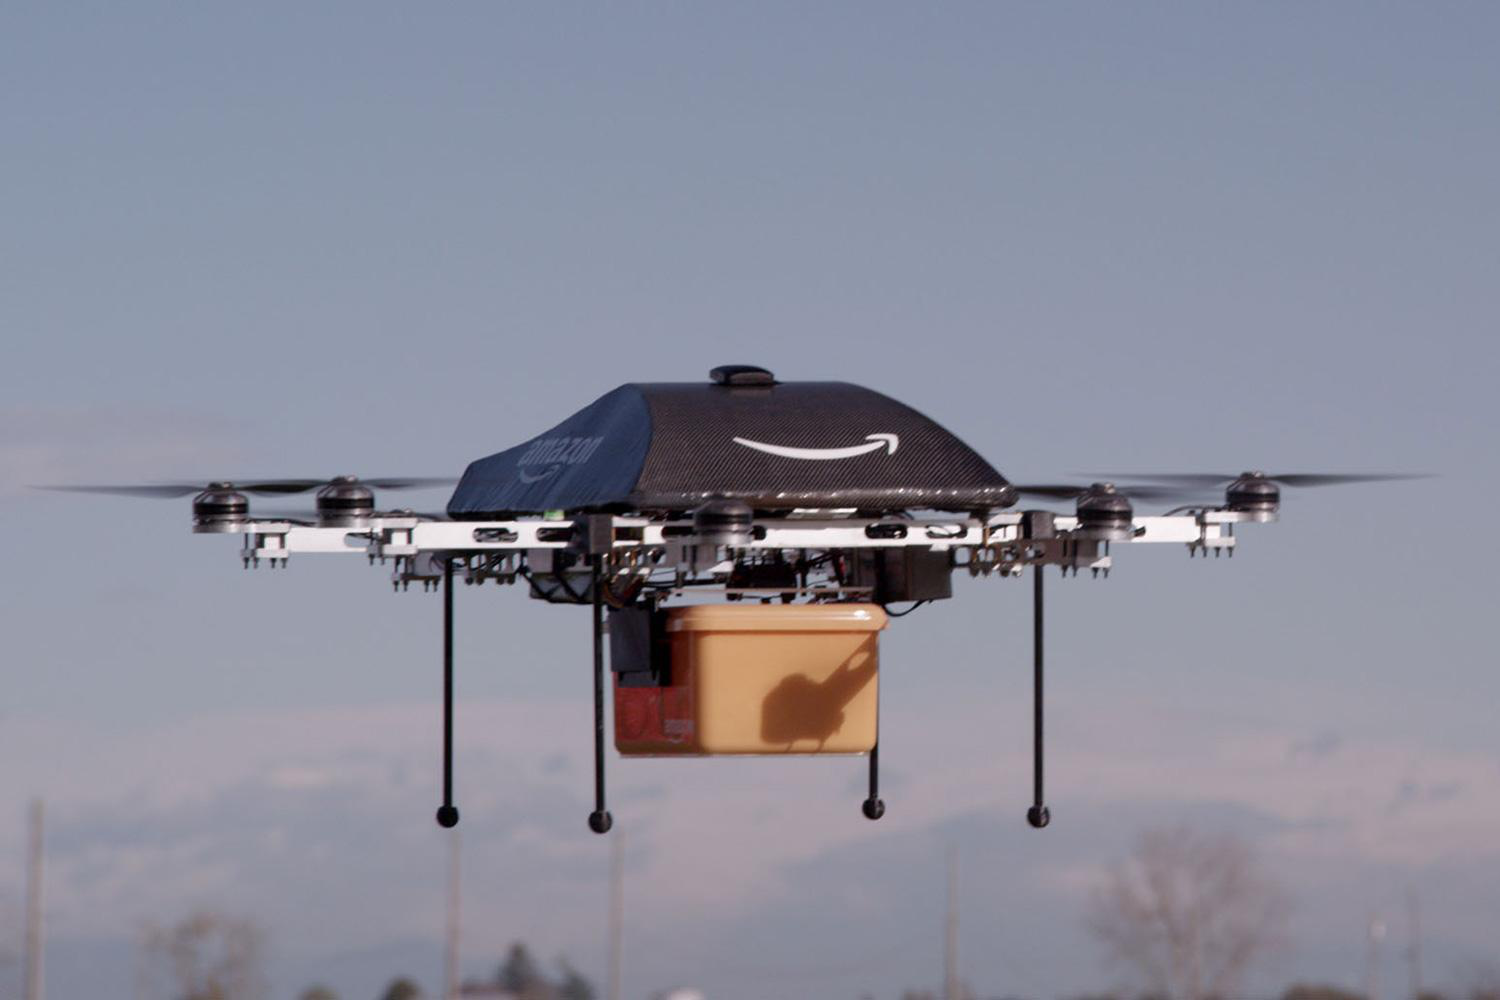
\includegraphics[scale=0.2]{immagini/amazon-air.png}
\caption{Drone della società statunitense Amazon. Consegnerà prodotti a domicilio in completa autonomia} 
\end{figure}
La nostra tesi si concentra proprio sull'applicazione ad un robot autonomo dei 
concetti di visione artificiale appena descritti.

